\documentclass[12pt, a4paper]{article}
\usepackage[margin=3cm]{geometry}
\usepackage{hyperref}
\usepackage[italian]{babel}
\usepackage{background}
\usepackage{graphicx}
\usepackage{soul}

\hypersetup{
    colorlinks=true,
    linkcolor=orange,
    filecolor=orange,
    urlcolor=orange,
    pdftitle={Ringraziamenti e Scuse},
    pdfauthor={Tommaso Bocchietti}
    }

\urlstyle{same}

\graphicspath{{./img/}{./pdf/}}

\backgroundsetup{
    scale=1,
    opacity=0.01,
    angle=0,
    contents={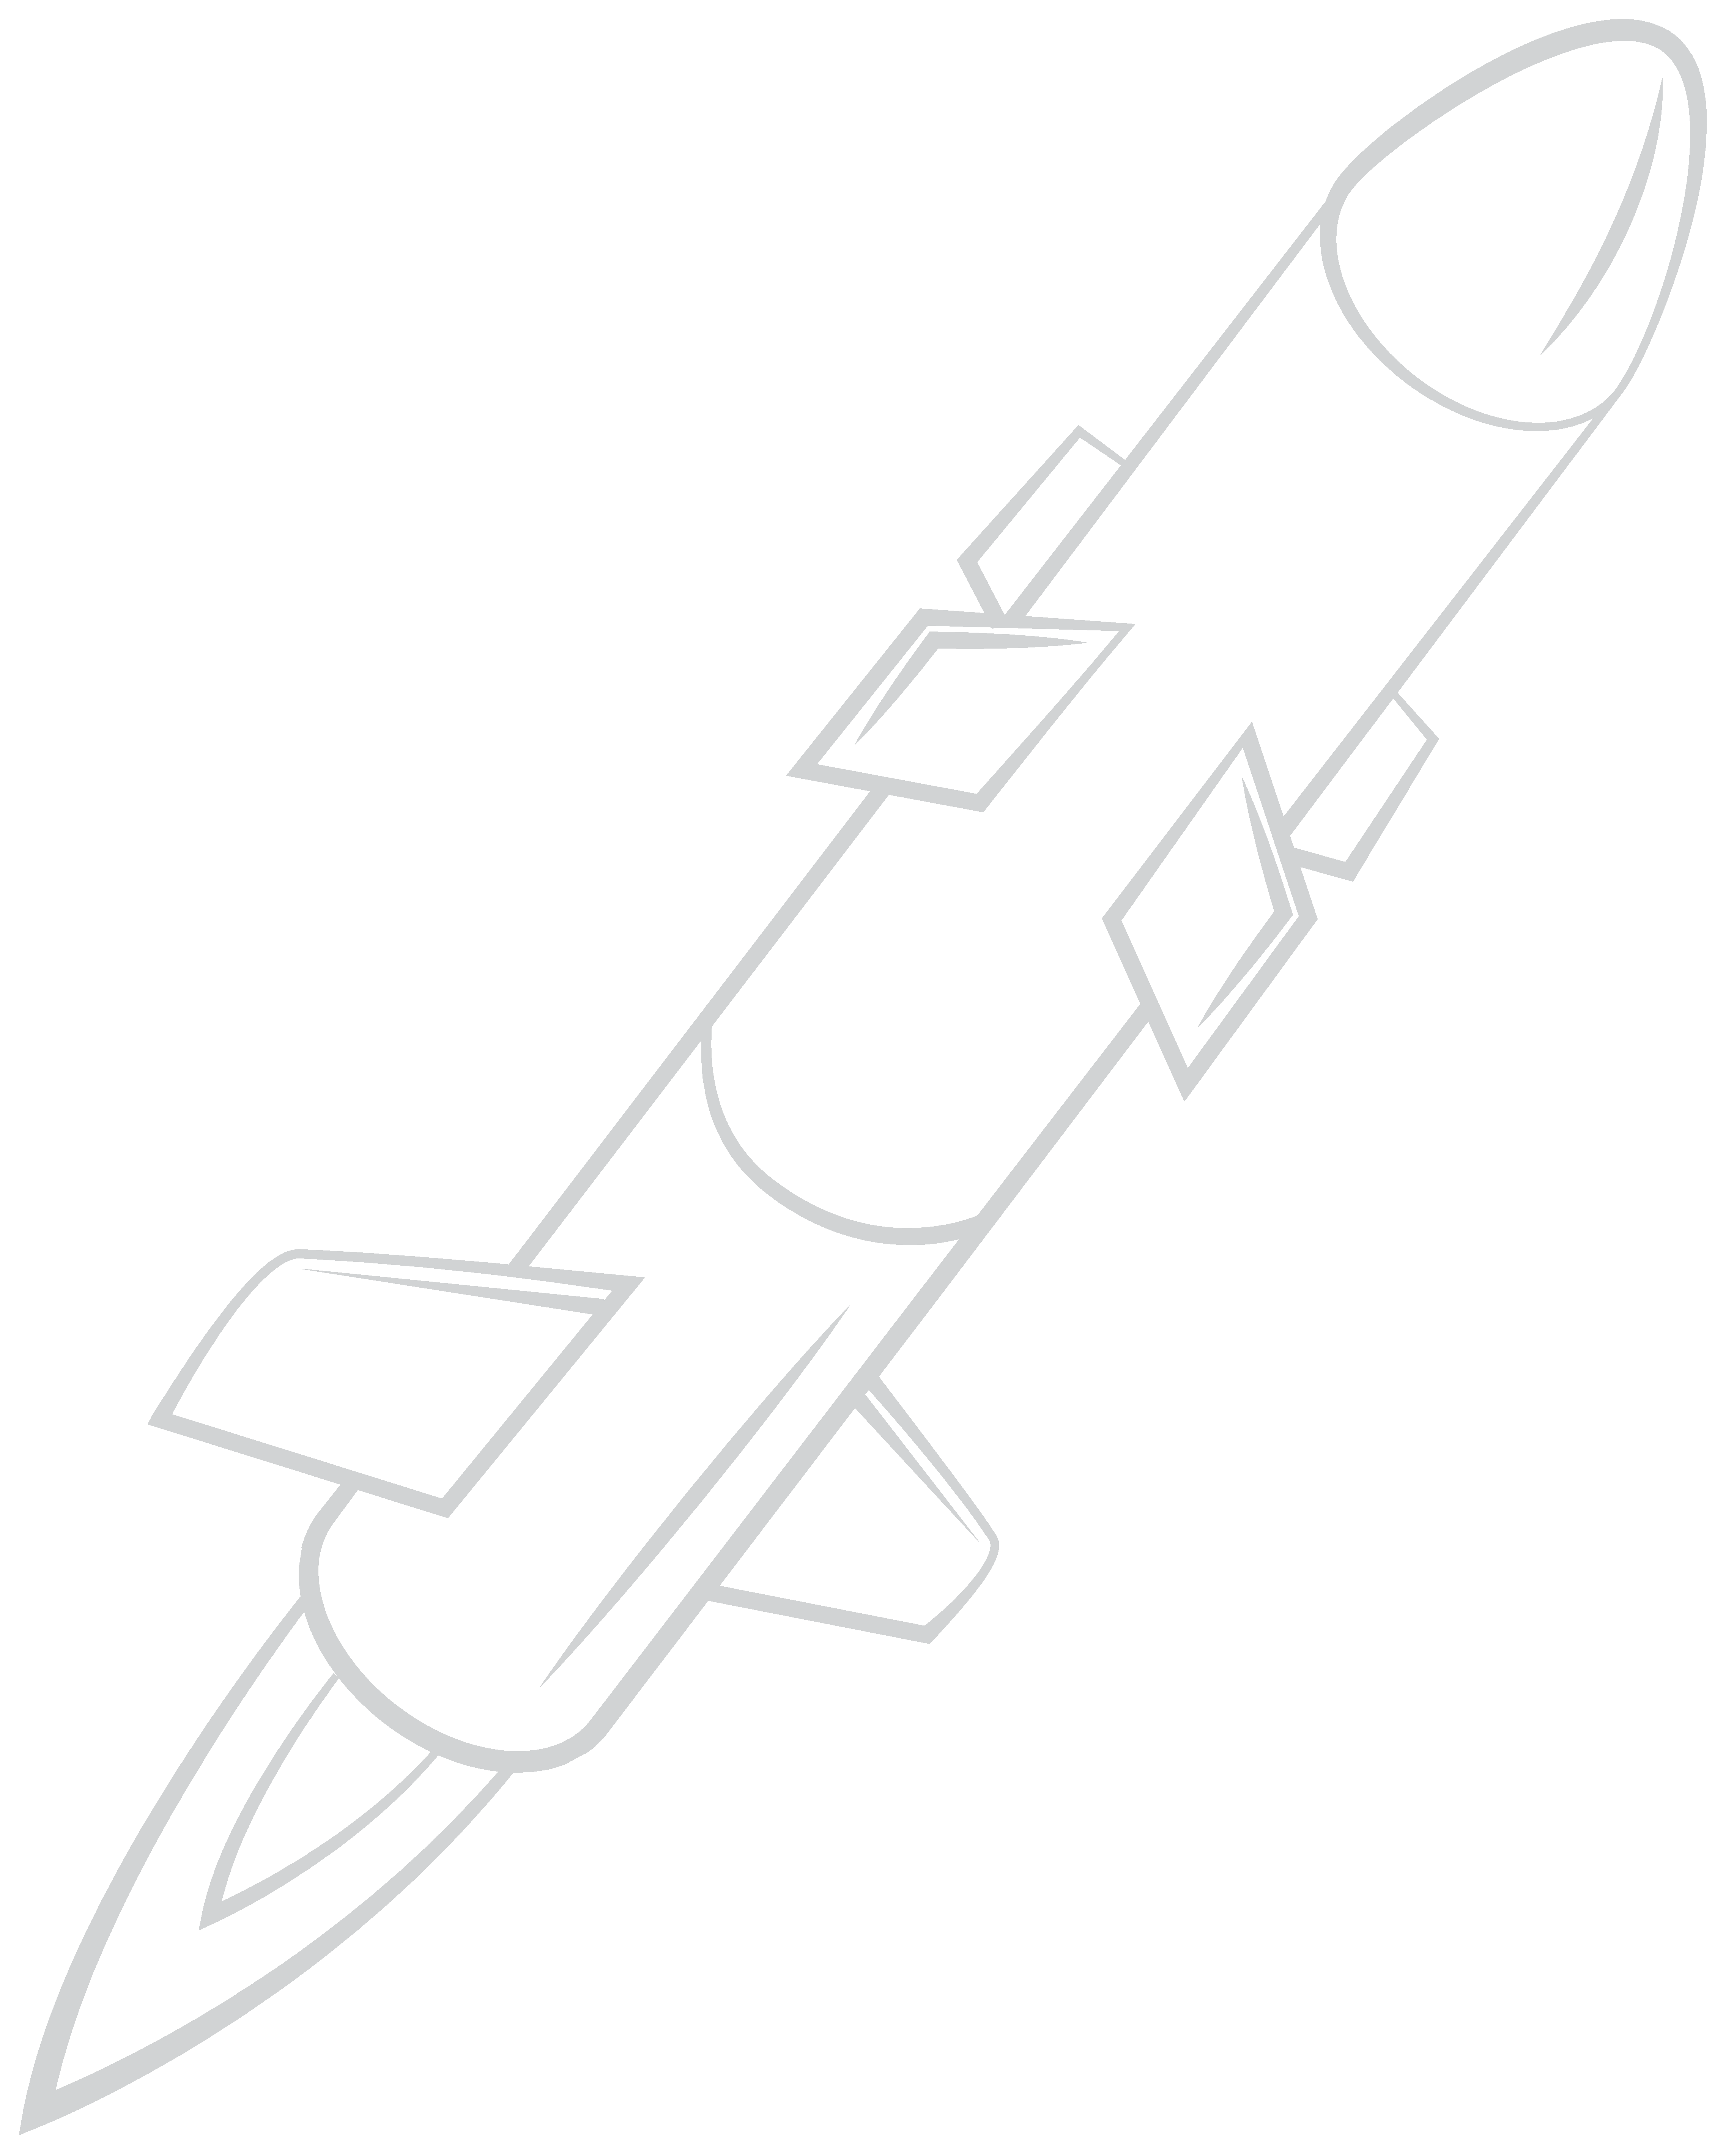
\includegraphics[width=0.6\paperwidth]{Rocket background.pdf}}
}

\begin{document}

\parbox{.35\linewidth}
{
    \begin{flushleft}
        
\includegraphics[width=2cm]{Gear bulb icon.png}\\
        % 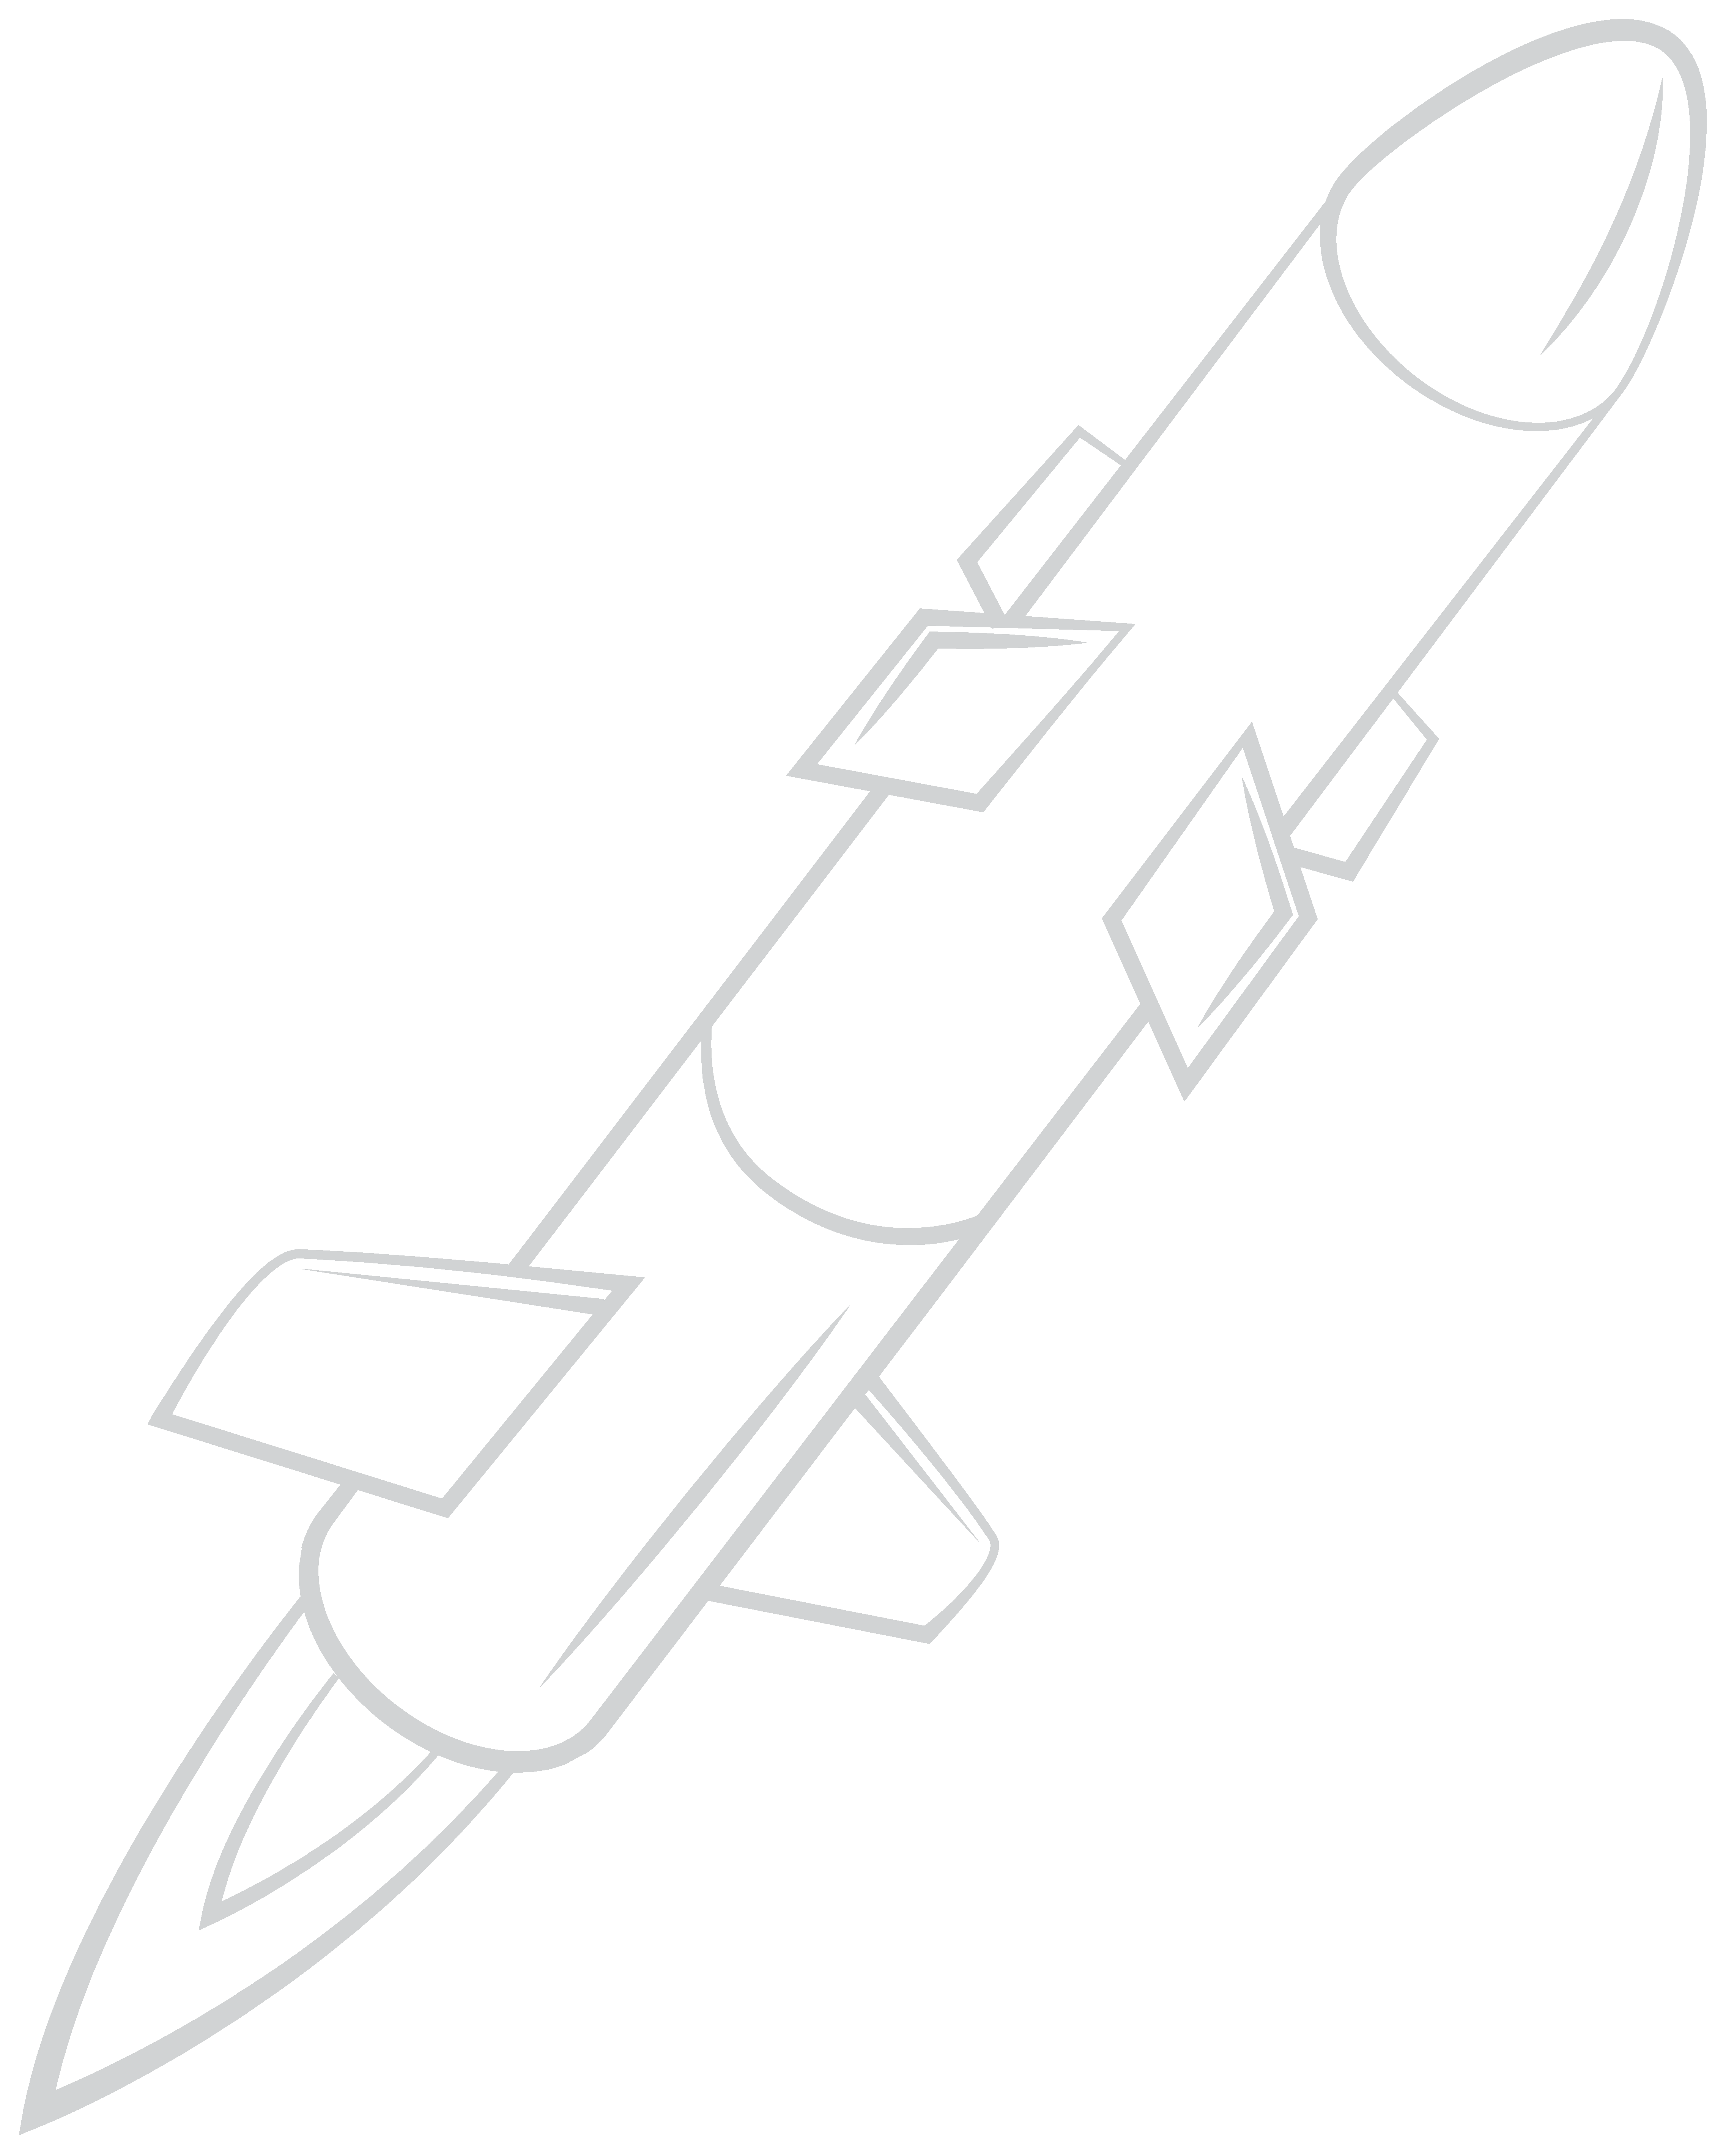
\includegraphics[width=2cm]{Rocket background.pdf}\\
    \end{flushleft}
}
\parbox{.6\linewidth}
{
    \begin{flushright}
        Laboratorio di Bocchio \\
        Sezione Aeronautica e Spazio profondo \\
        \vspace{1em}
        \today \\
    \end{flushright}
}

\vspace{3em}

\noindent A tutti coloro che ieri erano in cima alla montagna con il sottoscritto \\

% Letter style
\setlength{\parindent}{0pt}
\setlength{\parskip}{1.5em}

Non so neanche bene come impostarla questa lettera, quindi cercherò di far parlare più il mio io interiore e meno il mio cervello. Nelle successive righe sono previsti errori logici e incongruenze di vario tipo date dalla spontaneità della scrittura.

A ogni modo, questo breve messaggio vuole avere due fini, uno di ringraziamenti e uno di dovute scuse.

\textbf{Ringraziamenti}

Innanzitutto, grazie a tutti quelli che hanno deciso di venire e si sono magari sbattuti per organizzarsi a venire. Grazie davvero, vi voglio bene :).

Ringrazio poi tutti quelli che mi hanno sopportato durante la realizzazione del progetto, e in particolare @Bebbe, @Tetta e @Sergio.
Sostanzialmente negli ultimi 10 giorni gli continuavo a rompere le balle chiedendo e cercando riscontri e pareri. Grazie per la pazienza.

Ringraziamenti obbligatori poi per tutta la cerchia più ristretta di voi che sostanzialmente nelle ultime ore pre-lancio \st{mi hanno aiutato a organizzare} hanno organizzato tutto quello che era fuori dal puro tecnicismo legato ai razzi. Mi sarò anche laureato in Ingegneria Meccanica, ma il mio livello organizzativo è circa paragonabile a quello di un bambino di 5 anni.

\textbf{Scuse}

E mo qui ci divertiamo.

Allora, sinceramente me ne sono reso conto solo troppo tardi del casino che ho combinato ieri sera/notte. Sono stato abbastanza troppo egoista e non sono riuscito a ragionare in maniera oggettiva su come il mio comportamento stesse portando a una situazione di disagio per tutti.

Come sapete, ho questo piccolo difetto che se mi concentro e/o mi impunto su una cosa, di tutto quello che mi succede intorno non me ne accorgo. Anche se per ieri sera il verbo `accorgere' è meglio sostituibile con `interessare'.

Eravate tutti parte integrante della serata e io non mi sono mai reso conto del disagio che stavo causando ad ognuno di voi con il mio comportamento. E questo adesso mi fa abbastanza star male. Scusatemi.

Ogni tanto dimentico che, come mi dite sempre anche voi, ho una resistenza (non trovo un termine migliore al momento) maggiore rispetto alla media e ho sempre difficoltà nel ragionare immedesimandomi in un `non-Tommaso-Bocchietti' per capire come si possa reagire o cosa si possa provare in determinate situazioni.

Forse non si è capito niente dall'ultima frase, ma il concetto più pratico è che vedervi mezzi sonnambuli alla guida e/o sapere che avevate degli impegni il giorno successivo e per causa mia vi ho costretto a fare un `tour de force' vista la mia negligenza nel decidere subito di lasciar perdere e tornare a casa, mi fa sentire abbastanza in colpa.

Se vogliamo ricercare la causa di questo mio modo di fare, probabilmente è dovuto al fatto che sono troppo abituato a fare le cose da solo e per testa mia e non mi rendo conto che quando si è in gruppo bisogna anche ascoltare gli altri e non solo fare quello che si vuole.

Permettetemi quindi di concludere questo messaggio con quella che vuole essere una frase per strappare un mezzo sorriso perché misà che alla fine questa lettera è uscita fuori abbastanza pesante: non permettetemi mai più di andare con @Moscatello o un altro del gruppo di orientisti a completare una certa missione.
Alla fine se ci pensate, chi c'era sotto gli alberi a cercare di riprendere il razzo? @Io, @Moscatello, @Filibello e @Space :), che guarda caso siamo tutti orientisti. Coincidenze? Non credo.

\textbf{Nota:} l'ultima frase non vuole spartire la colpa della serata con gli altri orientisti, ma voleva essere solo un modo per sdrammatizzare e farvi sorridere un po'. Alla fine quello che li caricava a continuare a provarci e insistere ero sempre e solo io.

\textbf{Conclusioni}

In fin dei conti, spero solo di non aver incrinato i rapporti con nessuno di voi ma che al contrario questa folle avventura possa invece aver avuto modo di rafforzarli ancora di più.
Alla fine, quello che avete potuto osservare ieri è una versione di me che (per fortuna o purtroppo) mi rispecchia abbastanza bene in tutte le mie sfaccettature.
O meglio, diciamo che per rappresentami proprio al 100\%, a quest'ora il razzo dovrebbe essere qui di fianco a me\dots ma potete starne certi che più prima che poi, ci ritorna.

\begin{center}
    \huge E con i più intrepidi di voi,\\
    \textbf{ci vediamo alla prossima rampa di lancio!}
\end{center}

\end{document}
